\subsection{Inteligencia Artficial}
Definir a la inteligencia artificial llega a ser complicado, esto debido a la dificultad que se tiene en definir lo que en verdad es inteligencia. Algunos grandes personajes pensaban de la inteligencia como la ambición, mientras que otros mencionaban a la imaginación como gran impulsador de la inteligencia. También lo consideraban como la capacidad de adaptarse a los cambios. Estas definiciones hacen pensar que no existe un consenso claro de lo que es la inteligencia, menos aun de la inteligencia artificial; sin embargo, en términos generales, se puede calificar de “inteligencia artificial” a todo aquel sistema sintético que muestra algún tipo de comportamiento “inteligente”. Esto quiere decir que se puede considerar como IA a todo a aquellos que simule los sentidos naturales como el visión o audición, incluso a la capacidad de algunos sistemas de aprender de forma autónoma según su entorno lo requiera. \parencite{bk_hurbans2020grokking}

\subsection{Perceptrón}
Inventado por Frank Rosenblatt en 1957, el Perceptrón es la unidad básica de una red neuronal e incluso es considerado como la más simple red neuronal artificial (ANN). \parencite{bk_geron2022handml}

\begin{figure}[H]
	\begin{center}
		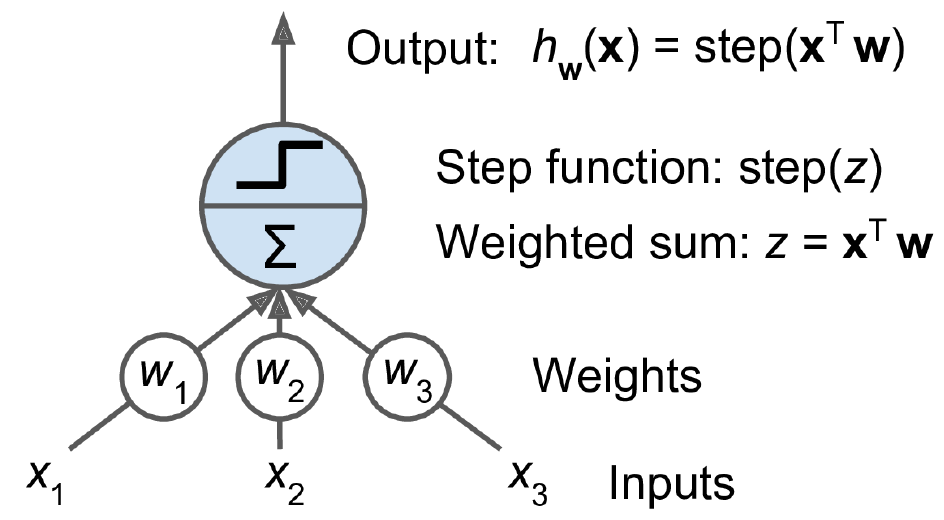
\includegraphics[width=1.00\textwidth]{2/figures/perceptron.png}
		\caption[Perceptrón]{Perceptrón. \\
		Fuente: \cite{bk_geron2022handml}. \textit{Hands-on machine learning with Scikit-Learn, Keras, and TensorFlow}.}
		\label{2:fig207}
	\end{center}
\end{figure}


\subsection{Perceptrón Multicapa}
Un Multi-Layer Perceptron (MLP) consiste en la unión de varios perceptrones, con la característica de estar organizados por capas. Existe una capa de entrada y otra de salida, todas las capas, a excepción de la salida, contiene una neurona adicional llamada bias. \parencite{bk_geron2022handml}

\begin{figure}[H]
	\begin{center}
		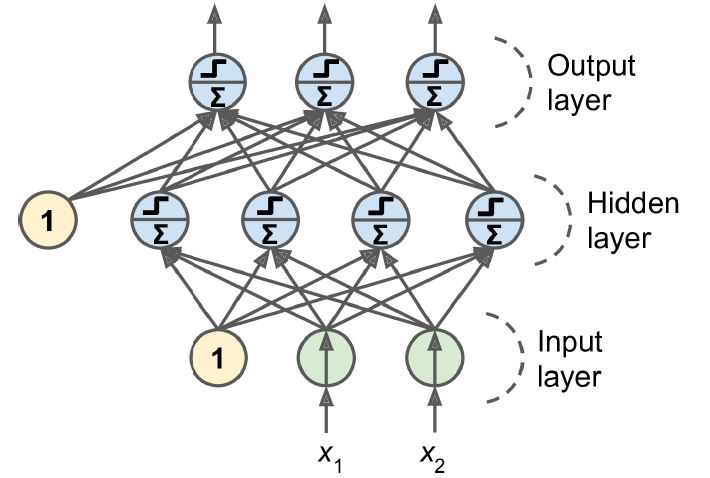
\includegraphics[width=1.00\textwidth]{2/figures/mlp.png}
		\caption[Perceptrón multicapa]{Perceptrón multicapa. \\
		Fuente: \cite{bk_geron2022handml}. \textit{Hands-on machine learning with Scikit-Learn, Keras, and TensorFlow}.}
		\label{2:fig208}
	\end{center}
\end{figure}


\subsection{Machine Learning}
El Aprendizaje Automático o Machine Learning es considerado como una ciencia y arte de dar instrucciones a una computadora para que pueda aprender por sí sola de una data. \parencite{bk_geron2022handml}

A continuación, se presenta el enfoque tradicional del Machine Learning.

\begin{figure}[H]
	\begin{center}
		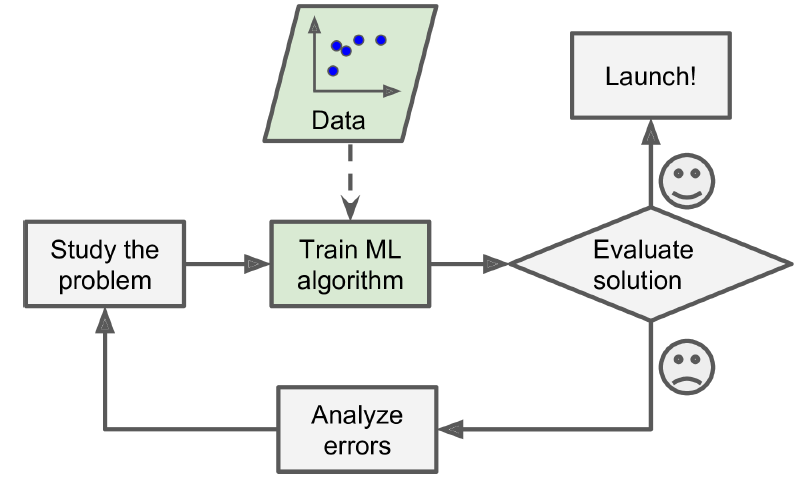
\includegraphics[width=1.00\textwidth]{2/figures/enfoque_ml.png}
		\caption[Enfoque del Machine Learning]{Enfoque del Machine Learning. \\
		Fuente: \cite{bk_geron2022handml}. \textit{Hands-on machine learning with Scikit-Learn, Keras, and TensorFlow}.}
		\label{2:fig209}
	\end{center}
\end{figure}

\subsection{Ecografía y las imágenes de ultrasonido}
Según \cite{pr_herrera2017diseimp}, la ecografía, que es una técnica de diagnóstico en donde se usan imágenes generadas por ultrasonido, es comúnmente desarrollado en las áreas de cardiología, ginecología, y otras más relacionadas. La popularidad de esta técnica se basa en la capacidad de las imágenes de alta calidad que se obtienen de este proceso, además de no ser un método invasivo o de radiación como muchos otros de su tipo.





